\section{Diseño del sistema aislado}\label{sec:aislado}

\subsection{Configuración del sistema}

El sistema es de respaldo: las cargas críticas se trasladan a un subtablero que se alimenta desde la salida del inversor-cargador. El generador fotovoltaico carga el banco de baterías por medio de un regulador MPPT, y el inversor-cargador convierte la energía del banco a \SI{120}{V} de corriente alterna. La red de JASEC llega a la entrada de corriente alterna del inversor-cargador; si el banco llega a su descarga máxima, la red alimenta las cargas y puede recargar el banco, y si la red falla, el equipo pasa las cargas al inversor. El sistema no entrega energía a la red.

\subsection{Balance de energía y capacidad del banco}\label{sec:balance}

La energía que debe entregar el generador se calculó con el método de balance de energía para sistemas aislados:
\begin{equation}
E_T = \frac{E_{CC}}{K_{TCC}} + \frac{E_{CA}}{K_{TCA}}, \qquad K_T = \left(1-\sum p\right)\left(1-\frac{K_a\,D}{\mathrm{DOD}}\right),
\end{equation}
donde $E_{CC}$ y $E_{CA}$ son las energías diarias de las cargas en corriente directa y alterna, $D$ los días de autonomía y $K_a$ la autodescarga diaria. Las pérdidas $p$ son valores típicos para sistemas aislados: cables 2\,\%, dispersión 4\,\%, suciedad 5\,\%, seguimiento del punto de máxima potencia 2\,\%, regulador 5\,\%, batería 1\,\% e inversor 5\,\%, este último solo para las cargas en alterna, con $K_a=0.005$. Con $D=2$ y $\mathrm{DOD}=0.7$ se obtiene $K_{TCA}=0.749$. Como todas las cargas son de alterna, $E_T = \SI{4334.5}{Wh}/0.749 = \SI{5786}{Wh}$ por día.

La capacidad del banco es
\begin{equation}
Q = \frac{1.1\,E_T\,D}{V\cdot\mathrm{DOD}} = \frac{1.1\cdot5786\cdot2}{24\cdot0.7} = \SI{758}{Ah},
\end{equation}
donde el factor 1.1 es el margen de seguridad del método. Con la batería seleccionada, de \SI{200}{Ah}, se requieren cuatro en paralelo, \SI{800}{Ah} y \SI{20.48}{kWh} nominales, que es el máximo que admite el fabricante \cite{pq_manual}. Al 70\,\% de descarga el banco entrega $24\cdot800\cdot0.7=\SI{13.44}{kWh}$, que alcanzan para 2.3 días de $E_T$. Esta autonomía supone que el banco está lleno cuando empieza el corte. Como el banco también alimenta las cargas en días normales, si el corte llega después de que el banco entregó la energía de un día completo quedan $13.44-4.56=\SI{8.88}{kWh}$, unos 1.5 días. En un día normal, si toda la energía de las cargas sale del banco, la descarga es de \SI{4334.5}{Wh}$/(0.95\cdot\SI{20480}{Wh})=22.3$\,\%.

La corriente máxima de cada batería es de \SI{200}{A} continuos \cite{pq_manual}. Con las cargas críticas encendidas a la vez, la corriente del banco es $I=P/(V\,(1-p_i))=783/(24\cdot0.95)=\SI{34.3}{A}$, y en el arranque de los compresores, \SI{77.3}{A}: ambas son mucho menores que los \SI{800}{A} que admiten las cuatro baterías en paralelo.

\subsection{Generador fotovoltaico}

La potencia del generador se calculó con la irradiación del peor mes sobre la cara este, noviembre, con \SI{3.73}{HSP} (Tabla~\ref{tab:radiacion}):
\begin{equation}
P_{\mathrm{campo}} = \frac{E_T}{\mathrm{HSP}} = \frac{5786}{3.73} = \SI{1551}{W}, \qquad N = \frac{1.1\,P_{\mathrm{campo}}}{P_{\mathrm{mod}}} = \frac{1.1\cdot1551}{450} = 3.79,
\end{equation}
de modo que se requieren cuatro módulos, \SI{1800}{Wp}. Ocupan \SI{8.0}{m^2} y pesan \SI{86}{kg}, y caben en una fila de cuatro módulos en vertical sobre la cara este, que mide \SI{4.7}{m} sobre la pendiente y \SI{9.2}{m} de largo.

\subsection{Conexión de los módulos en serie y en paralelo}

La cantidad máxima de módulos en serie se estima con $N_{\mathrm{serie}}=V_{\max,\mathrm{reg}}/V_{mp}=145/33.70=4.3$. Con la tensión de circuito abierto a \SI{7}{\celsius}, el límite es más estricto: $145/42.30=3.4$, es decir, hasta tres módulos en serie. Por otro lado, el regulador seleccionado arranca cuando la tensión fotovoltaica supera la del banco en \SI{5}{V} \cite{victron_mppt}; con la tensión de absorción de \SI{28.8}{V}, la tensión de máxima potencia del arreglo debe superar \SI{33.8}{V} aun con la celda a \SI{63.2}{\celsius}, donde un módulo da \SI{29.70}{V}. Se necesitan, por tanto, al menos dos módulos en serie. Con cuatro módulos, la única configuración posible es de dos cadenas de dos módulos (2S2P). La Tabla~\ref{tab:arreglo} resume sus valores.

\begin{table}[!htb]
\caption{Valores del arreglo 2S2P y límites del regulador}
\label{tab:arreglo}
\centering
\footnotesize
\setlength{\tabcolsep}{4pt}
\begin{tabular}{l c c}
\toprule
Parámetro & Arreglo & Límite del regulador \\
\midrule
$V_{oc}$ a \SI{7}{\celsius} & \SI{84.6}{V} & \SI{145}{V} (\SI{150}{V} absoluto) \\
$V_{mp}$ a \SI{7}{\celsius} & \SI{71.2}{V} & -- \\
$V_{mp}$ a \SI{63.2}{\celsius} & \SI{59.4}{V} & mayor que \SI{33.8}{V} \\
$I_{sc}$ a \SI{63.2}{\celsius} & \SI{28.8}{A} & \SI{70}{A} \\
$I_{mp}$ a \SI{63.2}{\celsius} & \SI{27.2}{A} & -- \\
Potencia en STC & \SI{1800}{W} & \SI{2400}{W} nominales a \SI{24}{V} \\
\bottomrule
\end{tabular}
\end{table}

\subsection{Regulador de carga}

La corriente del regulador debe ser
\begin{equation}
i_{\mathrm{reg}} \geq \frac{P_{\max}}{V_{\mathrm{bat}}} = \frac{1800}{24} = \SI{75}{A}.
\end{equation}
Se seleccionó el regulador MPPT Victron SmartSolar 150/85-Tr VE.Can, cuyas características están en la Tabla~\ref{tab:regulador}. Su corriente de \SI{85}{A} cumple el criterio; el modelo 150/70 de la misma serie, de \SI{70}{A}, no lo cumple. Además, es de seguimiento del punto de máxima potencia (MPPT), lo que permite conectar los módulos en serie con una tensión mayor que la del banco; selecciona automáticamente \SI{24}{V} y tiene un algoritmo de carga para baterías de litio, con la tensión de absorción de \SI{28.8}{V} que pide el fabricante de la batería \cite{victron_mppt, pq_manual}, y es del mismo fabricante que el inversor-cargador y se comunica con él, de modo que el sistema se puede supervisar desde una sola aplicación.

\begin{table}[!htb]
\caption{Características del regulador Victron SmartSolar MPPT 150/85-Tr VE.Can \cite{victron_mppt}}
\label{tab:regulador}
\centering
\footnotesize
\begin{tabular}{l l}
\toprule
Parámetro & Valor \\
\midrule
Tensión del banco & 12/24/48 V, selección automática \\
Corriente máxima de carga & \SI{85}{A} \\
Potencia FV nominal a \SI{24}{V} & \SI{2400}{W} \\
Corriente de cortocircuito FV máxima & \SI{70}{A} \\
Tensión FV máxima & \SI{150}{V} absoluta, \SI{145}{V} de operación \\
Tensión mínima de arranque & $V_{\mathrm{bat}}+\SI{5}{V}$ \\
Eficiencia máxima & 98\,\% \\
Absorción y flotación a \SI{24}{V} & \SI{28.8}{V} y \SI{27.6}{V} (ajustables) \\
Temperatura de operación & $-30$ a \SI{60}{\celsius} (plena potencia hasta \SI{40}{\celsius}) \\
Altitud máxima & \SI{5000}{m} (plena potencia hasta \SI{2000}{m}) \\
Terminales FV y de batería & \SI{35}{mm^2} (2 AWG) \\
Masa & \SI{4.5}{kg} \\
\bottomrule
\end{tabular}
\end{table}

La ficha garantiza la potencia plena hasta \SI{2000}{m} de altitud y el sitio está a \SI{2317}{m}. El arreglo tiene \SI{1800}{W}, el 75\,\% de la potencia nominal del regulador a \SI{24}{V}, y la corriente real hacia el banco es de $1800\cdot0.98/28.8=\SI{61.3}{A}$, el 72\,\% de su capacidad, de modo que una reducción de la potencia por altitud no limitaría la carga. La ficha no indica cuánto se reduce la potencia por encima de \SI{2000}{m}, por lo que conviene confirmarlo con el fabricante.

\subsubsection{Área de operación segura}

La Fig.~\ref{fig:soa} muestra la zona en que puede operar el regulador, limitada por la tensión mínima de arranque, la tensión máxima de \SI{145}{V} y la corriente de cortocircuito de \SI{70}{A}, junto con las curvas I-V del arreglo 2S2P a 7, 25 y \SI{63.2}{\celsius}. Las curvas se trazaron con el modelo exponencial de cuatro parámetros de la ficha ($V_{oc}$, $I_{sc}$, $V_{mp}$, $I_{mp}$). Los puntos de máxima potencia quedan entre 59.4 y \SI{71.2}{V} y cerca de \SI{27}{A}, dentro de la zona de operación, y la tensión de circuito abierto en frío, \SI{84.6}{V}, queda \SI{60.4}{V} por debajo del límite de operación.

\begin{figure}[!htb]
\centering
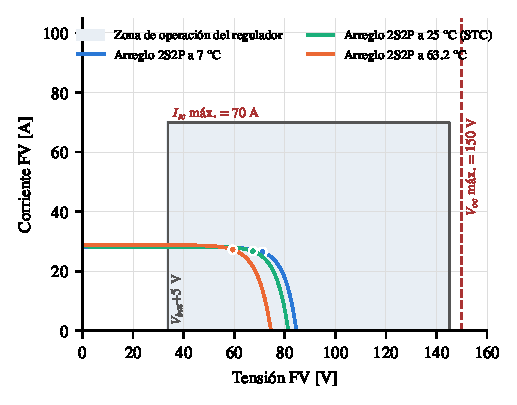
\includegraphics[width=\anchofig]{soa_regulador.pdf}
\caption{Zona de operación del regulador y curvas I-V del arreglo 2S2P a distintas temperaturas de celda. Los puntos marcan la máxima potencia.}
\label{fig:soa}
\end{figure}

\subsection{Inversor-cargador}

El inversor de un sistema aislado se dimensiona con la potencia de las cargas de alterna que funcionan a la vez, debe soportar los picos de arranque de los motores, que pueden ser de 3 a 4 veces la potencia nominal, y debe tener corte por baja tensión del banco. La tensión de entrada es la del banco y la de salida, la de las cargas. Con las cargas críticas, la potencia simultánea es de \SI{783}{W} y el pico con el arranque de los dos compresores, de \SI{1763}{W} (Sección~\ref{sec:lugar}).

Se seleccionó el inversor-cargador Victron MultiPlus-II 24/3000/70-50 de \SI{120}{V}, cuyas características están en la Tabla~\ref{tab:inversor}. Las cargas usan el 33\,\% de su potencia continua a \SI{25}{\celsius} y el 32\,\% de su potencia pico. Es el modelo de menor potencia de la serie MultiPlus-II para \SI{24}{V} y \SI{120}{V} \cite{victron_mp}. Incluye un conmutador de transferencia de \SI{50}{A}: si falla la red, pasa las cargas al inversor en menos de \SI{20}{ms}, de modo que los equipos electrónicos siguen funcionando sin interrupción. También incluye un cargador de \SI{70}{A}, que puede recargar el banco desde la red cuando la energía solar no alcanza, y protección por baja tensión del banco \cite{victron_mp}. Su salida es de onda senoidal, apta para los compresores y para los equipos electrónicos.

\begin{table}[!htb]
\caption{Inversor-cargador Victron MultiPlus-II 24/3000/70-50 120V \cite{victron_mp} frente a las cargas}
\label{tab:inversor}
\centering
\footnotesize
\setlength{\tabcolsep}{3pt}
\begin{tabular}{l l l}
\toprule
Parámetro & Cargas críticas & Inversor-cargador \\
\midrule
Potencia continua & \SI{783}{W} & \SI{2400}{W} a \SI{25}{\celsius}; \SI{2200}{W} a \SI{40}{\celsius} \\
Potencia pico & \SI{1763}{W} & \SI{5500}{W} \\
Tensión de entrada DC & \SI{24}{V} & 19 a \SI{33}{V} \\
Salida AC & \SI{120}{V}, \SI{60}{Hz} & \SI{120}{V} $\pm$ 2\,\%, \SI{60}{Hz} \\
Corriente de batería & \SI{34.3}{A} (\SI{77.3}{A} en el arranque) & \\
Conmutador de transferencia & & \SI{50}{A}, menos de \SI{20}{ms} \\
Cargador desde la red & & \SI{70}{A}; absorción \SI{28.8}{V}, flotación \SI{27.6}{V} \\
Eficiencia máxima & & 94\,\% \\
Consumo sin carga & & \SI{13}{W} (\SI{3}{W} en modo de búsqueda) \\
Temperatura de operación & & $-40$ a \SI{60}{\celsius} \\
Masa & & \SI{19}{kg} \\
\bottomrule
\end{tabular}
\end{table}

El consumo sin carga del inversor, de \SI{13}{W}, equivale a \SI{312}{Wh} por día si funciona sin interrupción, más que los \SI{217}{Wh} por día que representa la pérdida de 5\,\% del inversor en el balance. La diferencia, de \SI{95}{Wh} por día, queda cubierta por el excedente de \SI{697}{Wh} por día de noviembre (Tabla~\ref{tab:energia}), y se reduce si se activa el modo de búsqueda del equipo, de \SI{3}{W}.

\subsection{Estimación energética}

La energía diaria disponible para las cargas se estimó para cada mes como $E = P_{\mathrm{campo}}\cdot\mathrm{HSP}\cdot K_{TCA}$, con los \SI{1.8}{kW} del arreglo, la irradiación de la cara este y el mismo factor de rendimiento del balance. La Tabla~\ref{tab:energia} y la Fig.~\ref{fig:energia} comparan esa energía con la demanda de las cargas críticas.

\begin{table}[!htb]
\caption{Energía mensual disponible y demanda de las cargas críticas}
\label{tab:energia}
\centering
\footnotesize
\setlength{\tabcolsep}{4pt}
\begin{tabular}{l c r r r r}
\toprule
Mes & HSP & Generada [kWh] & Disponible [kWh] & Demanda [kWh] & Cobertura \\
\midrule
Ene & 5.03 & 280.7 & 210.3 & 134.4 & 156\,\% \\
Feb & 5.73 & 288.8 & 216.3 & 121.4 & 178\,\% \\
Mar & 5.94 & 331.5 & 248.3 & 134.4 & 185\,\% \\
Abr & 5.54 & 299.2 & 224.1 & 130.0 & 172\,\% \\
May & 4.55 & 253.9 & 190.2 & 134.4 & 142\,\% \\
Jun & 4.36 & 235.4 & 176.4 & 130.0 & 136\,\% \\
Jul & 4.35 & 242.7 & 181.8 & 134.4 & 135\,\% \\
Ago & 4.51 & 251.7 & 188.5 & 134.4 & 140\,\% \\
Set & 4.49 & 242.5 & 181.6 & 130.0 & 140\,\% \\
Oct & 3.94 & 219.9 & 164.7 & 134.4 & 123\,\% \\
Nov & 3.73 & 201.4 & 150.9 & 130.0 & 116\,\% \\
Dic & 4.46 & 248.9 & 186.4 & 134.4 & 139\,\% \\
\midrule
Año & & 3096 & 2320 & 1582 & 147\,\% \\
\bottomrule
\end{tabular}
\\[2pt]
{\footnotesize Generada: $P_{\mathrm{campo}}\cdot\mathrm{HSP}\cdot\text{días}$. Disponible: generada por $K_{TCA}=0.749$.}
\end{table}

\begin{figure}[!htb]
\centering
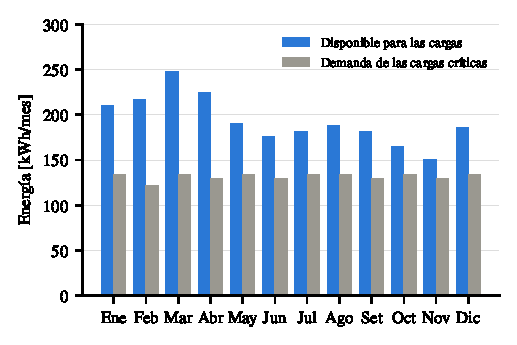
\includegraphics[width=\anchofig]{energia_mensual.pdf}
\caption{Energía mensual disponible para las cargas y demanda de las cargas críticas.}
\label{fig:energia}
\end{figure}

Todos los meses la energía disponible supera la demanda: en noviembre, el mes de diseño, la cobertura es de 116\,\%, y en marzo llega a 185\,\%. En el año hay \SI{2320}{kWh} disponibles para \SI{1582}{kWh} de demanda. El excedente no se aprovecha, porque el sistema no entrega energía a la red, pero permite recargar el banco después de días nublados: en noviembre el excedente medio es de \SI{0.70}{kWh} por día, de modo que recargar los \SI{13.44}{kWh} de los dos días de autonomía tomaría unos 19 días de radiación media, o menos si se usa el cargador desde la red. Como comparación, PVGIS estima para \SI{1.8}{kWp} en la cara este, con 14\,\% de pérdidas del sistema y las pérdidas por temperatura y ángulo de incidencia, \SI{2401}{kWh} al año y \SI{156}{kWh} en noviembre \cite{pvgis}, valores cercanos a la energía disponible estimada.
